\section{Continuous Spatial Dynamics}
The spatial tissue simulations discussed in this section are based on a
continuous approximation of the tissue, which in reality is composed of
discrete cells. The mathematical approach was introduced in section
\ref{sec:contdescr}. In practice - regardless of the specific model used - one
adds a diffusion term to the ODE describing the temporal evolution of the
membrane potential and obtains a parabolic PDE:
\begin{equation}
    \dv{V}{t}=G(V)\longrightarrow\dv{V}{t}=\eta\,\nabla^2{V}+G(V)
\end{equation}

In this case the - usually anisotropic - diffusivity is given by the scalar
coefficient $\eta$, which was set to $\eta=0.3$ in all cases presented below.
Additionally, the time step is computed in each case to fulfill the CFL
condition:
\begin{equation*}
    \Delta{t}<\frac{(\Delta{x})^2}{2\,\eta}
\end{equation*}


\subsection{On a one-dimensional domain}
The simulation was performed using the Aliev-Panfilov model. For the
calculations two one-dimensional arrays were used, representing the values of the membrane
potential and the relaxation variable along a discretized line, the length of
which has been varied throughout the simulations while holding the grid
spacing constant at $\Delta{x}=0.2$.

At the beginning von-Neumann boundary conditions were imposed and the first
value of the potential array was set to one. Then at each time step both arrays
were updated using a simple Euler scheme according to
\begin{align*}
    \dv{V}{t}&=\eta\,\pdv[2]{V}{x}+G_{V}(V, W) \\
    \dv{W}{t}&=G_{W}(V, W)
\end{align*}
where $G_V$ and $G_W$ are the right hand sides in \eqref{eq:ap_pot} and
\eqref{eq:ap_relax} respectively.

After sufficient steps for the peak of the action potential to develop, the
von-Neumann boundary conditions are replaced by periodic boundary
conditions, which mimics a regular succession of peaks at a constant rate.
This rate can be modified by changing the length of the line along which the
values are computed.

When performing the simulation for different lengths, one finds several
quantities of interest:
\begin{description}
    \item[Base Cycle Length] \emph{BCL}, the time for the peak to travel along
        the line one (or the time between two peaks, the period)
    \item[Conduction Velocity] \emph{CV}, Velocity of the peak (length of line
        divided by BCL)
    \item[Action Potential Duration] \emph{APD}, time between upstroke and
        downstroke
    \item[Rise Time] duration of upstroke
    \item[Maximal Peak Height]
\end{description}

These quantities were measured by monitoring a fixed point on the domain and
checking at each time step whether the potential crossed either a low or a high
threshold (5\% and 95\% of the maximal potential respectively).
The length of the domain was varied between 25 and 200 and for each value ten
measurements were recorded by letting the peak pass through the domain ten times after
reaching a stable form. Then average and standard deviation were computed and
plotted (see \figref{fig:alpha2}).

\begin{figure}[h]
    \centering
    \begin{subfigure}[b]{.3\textwidth}
        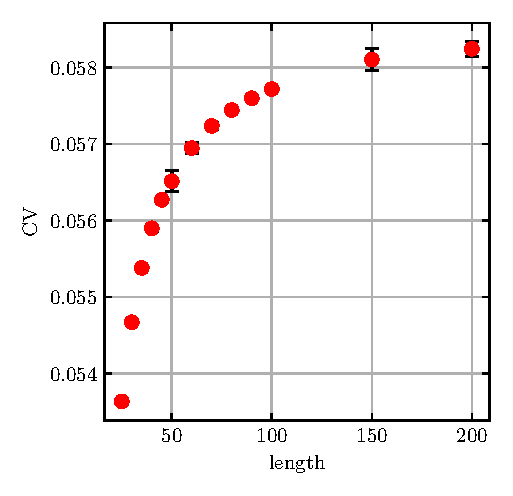
\includegraphics[width=\textwidth]{alpha-measurements-cv}
        \vspace{-\baselineskip}
        \label{fig:alpha-measure-cv}
        \caption{conduction velocity}
    \end{subfigure}
    \vspace{\baselineskip}
    ~
    \begin{subfigure}[b]{.3\textwidth}
        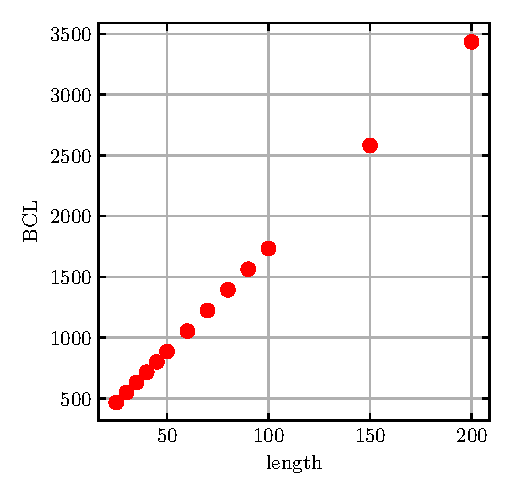
\includegraphics[width=\textwidth]{alpha-measurements-bcl}
        \vspace{-\baselineskip}
        \label{fig:alpha-measure-bcl}
        \caption{base cycle length}
    \end{subfigure}
    ~
    \begin{subfigure}[b]{.3\textwidth}
        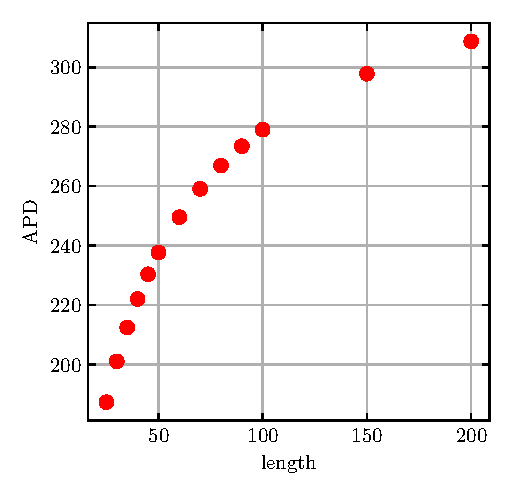
\includegraphics[width=\textwidth]{alpha-measurements-apd}
        \vspace{-\baselineskip}
        \label{fig:alpha-measure-apd}
        \caption{action potential duration}
    \end{subfigure}
    \begin{subfigure}[b]{.3\textwidth}
        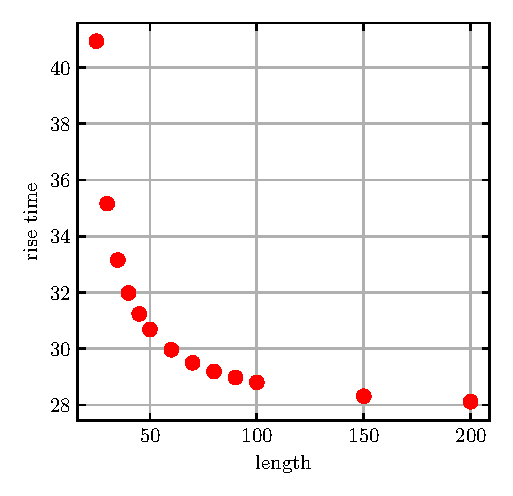
\includegraphics[width=\textwidth]{alpha-measurements-rt}
        \vspace{-\baselineskip}
        \label{fig:alpha-measure-rt}
        \caption{rise time}
    \end{subfigure}
    ~
    \begin{subfigure}[b]{.3\textwidth}
        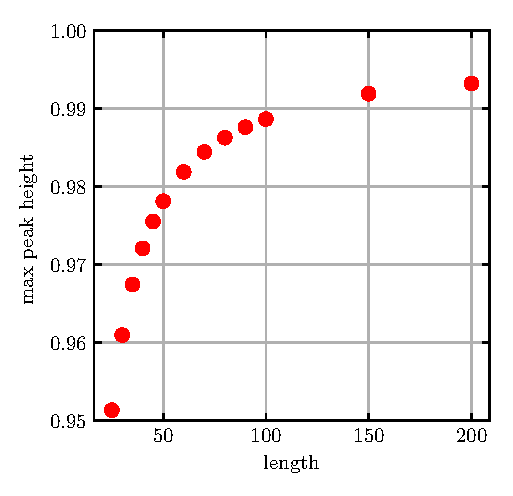
\includegraphics[width=\textwidth]{alpha-measurements-vmax}
        \vspace{-\baselineskip}
        \label{fig:alpha-measure-vmax}
        \caption{max peak height}
    \end{subfigure}
    \label{fig:alpha2}
    \caption{All measured quantities plotted against the domain length}
\end{figure}

Of course, the BCL increases linearly with the maximal length.  The CV and
maximal peak height have smaller values for small lengths, which corresponds to
a high rate of succeeding action potentials. With longer lengths, \ie~lower
rates, those values first increase strongly in value and then seem to strive
asymptotically against some upper limit (CV 0.0582, max peak: 0.9931).  The APD
seems to behave similarly, but to verify its asymptotic character, a closer
investigation is required.  The rise time is maximal for small lengths, then
falls and goes towards some lower limit. One can conclude therefrom, that the
action potentials rising edge is the most shallow for high rates and gets
steeper for lower rates.

Concerning the theoretical estimated relationship between CV and rise time
\begin{equation}
    CV\approx\sqrt{\frac{\eta}{2\tau}}(1-2\alpha)
    \label{eq:cvrt}
\end{equation}
the measured values were plotted in \figref{fig:alpha-cv-rt} together with the
curve given by \eqref{eq:cvrt} (where $\alpha=0.17$ was obtained by fitting the
measured data to the formula using a non-linear least squared method; this is
justified, since $\alpha$ acts only as an offset).

\begin{figure}[h]
    \centering
    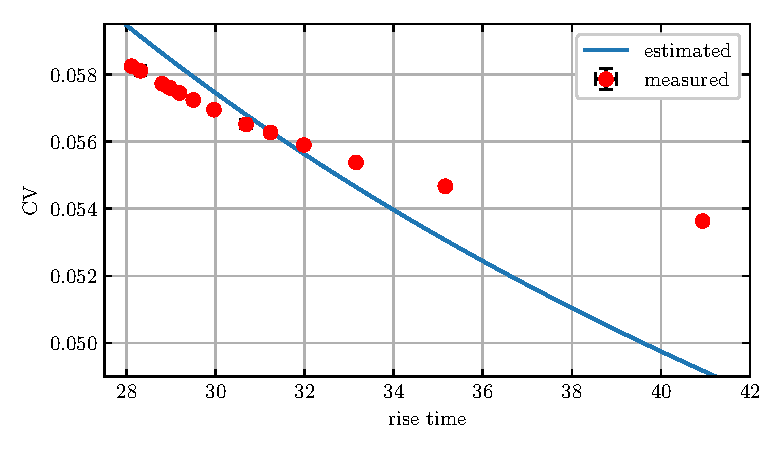
\includegraphics[width=.65\textwidth]{alpha-measurements-cv-rt}
    \label{fig:alpha-cv-rt}
    \caption{comparison of measurement and estimate}
\end{figure}

In order to (naively) quantize this result, both curves were approximated as
linear and a linear regression was computed (see table~\ref{tab:linreg}).
\begin{table}[h]
    \centering
    \begin{tabular}{l | c c}
        \toprule
        & {slope} & {$r^2$-value} \\
        \midrule
        \textbf{measured} & \num{-3.7e-4} & 0.92 \\
        \textbf{estimated} & \num{-7.7e-4} & 0.99 \\
        \bottomrule
    \end{tabular}
    \label{tab:linreg}
    \caption{Results of linear regression}
\end{table}
The relative error of the slopes is ca.~48\%.


\subsection{On a two-dimensional domain}
The setups described below were simulated with the Aliev-Panfilov model and
with the Fenton model. However hereafter only the results from the Fenton model
are presented, since while exhibiting the same phenomena as the
first-mentioned, it also shows some additional interesting features.

The Fenton simulation is based on three two-dimensional arrays holding the
spatially resolved values of the membrane potential and the two inactivation
gates. These arrays are update each time step with an Euler scheme according to
\begin{align*}
    \dv{V}{t}&=\eta\,\nabla^2{V}+G_{V}(V, v, w) \\
    \dv{v}{t}&=G_{v}(V, v, w) \\
    \dv{w}{t}&=G_{w}(V, v, w)
\end{align*}
where $G_V$, $G_v$ and $G_w$ are the right hand sides in \eqref{eq:cap},
\eqref{eq:v} and \eqref{eq:w} respectively.

All of the following setups used grid steps $\Delta{x}=\Delta{y}=1$. Varying
this parameter corresponds simply to a rescaling of the system.


\subsubsection{Channel}
One considers a $64\times256$ grid with Dirichlet boundary conditions imposed
along the long side (\ie~the x-direction) and periodic boundary conditions
along the short side (\ie~the y-direction).

For the initial values of $V$ and $w$ the same narrow stripe (20 grid points
wide) and for $v$ a stripe of same width but shifted 10 grid points in positive
x-direction were set to 1.

Running the simulation, an action potential quickly develps and repeatedly
passes through the domain, which mimics a constant rate of pulses. Because of
the Dirichlet conditions the action potential on the edges is pulled to zero,
causing some kind of tail (as shown in \figref{fig:pulse}).

\begin{figure}[h]
    \centering
    
\includegraphics[width=.75\textwidth]{fenton-cont-pulse}
    \label{fig:pulse}
    \caption{Pulse in channel setup}
\end{figure}


\subsubsection{Spiral Excitation}
Now one considers a $128\times512$ grid with von-Neumann boundary conditions
imposed on all sides. The initial conditions to generate the first pulse are
the same as described above. Because of the boundary conditions, the pulse is
not damped on the edges an passes through the domain only once.

Now a small area of $10\times10$ grid points right in the middle of the domain
has its membrane potential set to 1. In the absence of any prior excitation
this simply produces a circular pulse running away in all directions. But if
this perturbation happens in the wake of a preceding action potential an
interaction with the relaxation variables - which have not yet fully returned
to their rest values - takes place: Either the perturbation is suppressed right
away, or it is pushed backwards growing into the shape of an expanding
croissant whose edges are running forward until the meet in the
center. Upon this meeting the croissant becomes a pretzel which runs away in a
circular fashion and the then slightly inwards turned edges generate a new
croissant-shaped pulse which undergoes the same process.

\begin{figure}[h]
    \centering
    \begin{subfigure}[b]{.45\textwidth}
        
\includegraphics[width=\textwidth]{spiral-80}
        \vspace{-\baselineskip}
        \caption{2400 steps}
    \end{subfigure}
    \begin{subfigure}[b]{.45\textwidth}
        
\includegraphics[width=\textwidth]{spiral-81}
        \vspace{-\baselineskip}
        \caption{2430 steps}
    \end{subfigure}
    \begin{subfigure}[b]{.45\textwidth}
        
\includegraphics[width=\textwidth]{spiral-84}
        \vspace{-\baselineskip}
        \caption{2520 steps}
    \end{subfigure}
    \begin{subfigure}[b]{.45\textwidth}
        
\includegraphics[width=\textwidth]{spiral-87}
        \vspace{-\baselineskip}
        \caption{2610 steps}
    \end{subfigure}
    \begin{subfigure}[b]{.45\textwidth}
        
\includegraphics[width=\textwidth]{spiral-100}
        \vspace{-\baselineskip}
        \caption{3000 steps}
    \end{subfigure}
    \begin{subfigure}[b]{.45\textwidth}
        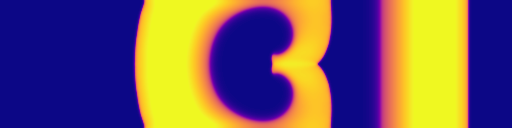
\includegraphics[width=\textwidth]{spiral-110}
        \vspace{-\baselineskip}
        \caption{3300 steps}
    \end{subfigure}
    \begin{subfigure}[b]{.45\textwidth}
        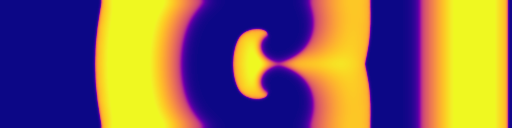
\includegraphics[width=\textwidth]{spiral-120}
        \vspace{-\baselineskip}
        \caption{3600 steps}
    \end{subfigure}
    \begin{subfigure}[b]{.45\textwidth}
        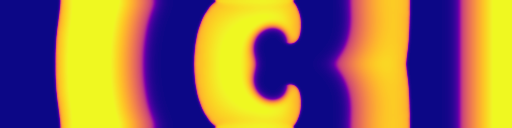
\includegraphics[width=\textwidth]{spiral-130}
        \vspace{-\baselineskip}
        \caption{3900 steps}
    \end{subfigure}
    \label{fig:spiral}
    \caption{Image series of spiral excitation due to well-timed perturbation}
\end{figure}

For the given setup, the sweet spot in insert this perturbation lies around
2430 integration steps (see \figref{fig:spiral}).

While with the Fenton model each succeeding spiral is slightly damped causing
the process to be extinguished completely after a finite number of iterations,
the spirals generated with the Aliev-Panfilov model do not seem to exhibit such
kind of behaviour and instead seem to go on indefinitely.


\subsubsection{Spiral Wave and Breakup}
Finally one considers a $256\times512$ grid with von-Neumann boundary
conditions on all sites. The initial conditions are given by a stripe of
excited membrane potential which only reaches into the domain by some extend,
\ie~it has a loose end.

When performing the simulation, the main part of the initial stripe develops
into a pulse like seen before, but the loose end turns away growing into a
spiral and eventually hits its own wake. When the tip reaches not yet fully
repolarized tissue, it fails to continue propagating normally and instead
breaks up (in the Fenton model this is due to the interaction of the action
potential of the tip with the inactivation gates in the wake). This process
starts to successively generate new spirals. It amplifies itself, soon causing
multiple spirals to be present at once, which spread out until the whole domain
is disruptively filled with small and rather fast moving spirals (see
\figref{fig:breakup}).

\begin{figure}[h]
    \centering
    \begin{subfigure}[b]{.3\textwidth}
        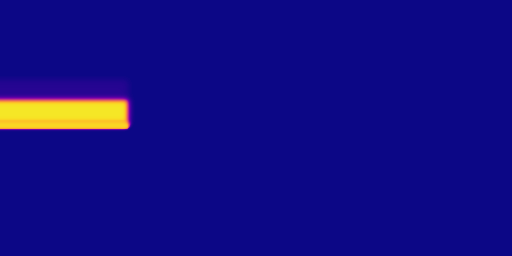
\includegraphics[width=\textwidth]{breakup-1}
        \vspace{-\baselineskip}
        \caption{50 steps}
    \end{subfigure}
    \begin{subfigure}[b]{.3\textwidth}
        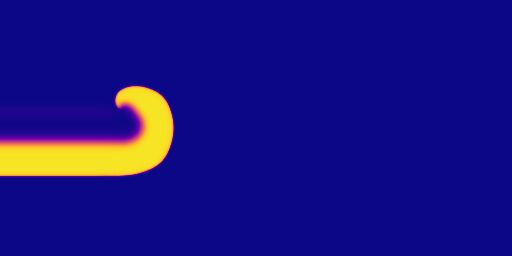
\includegraphics[width=\textwidth]{breakup-6}
        \vspace{-\baselineskip}
        \caption{300 steps}
    \end{subfigure}
    \begin{subfigure}[b]{.3\textwidth}
        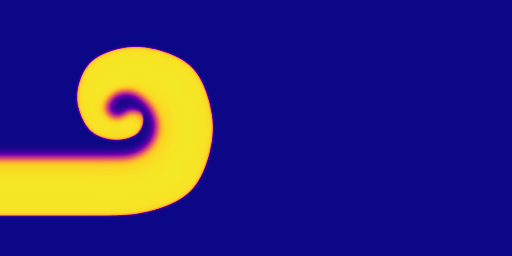
\includegraphics[width=\textwidth]{breakup-10}
        \vspace{-\baselineskip}
        \caption{500 steps}
    \end{subfigure}
    \begin{subfigure}[b]{.3\textwidth}
        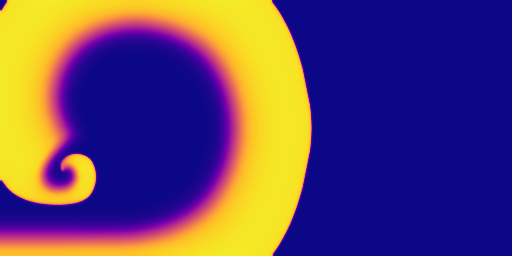
\includegraphics[width=\textwidth]{breakup-20}
        \vspace{-\baselineskip}
        \caption{1000 steps}
    \end{subfigure}
    \begin{subfigure}[b]{.3\textwidth}
        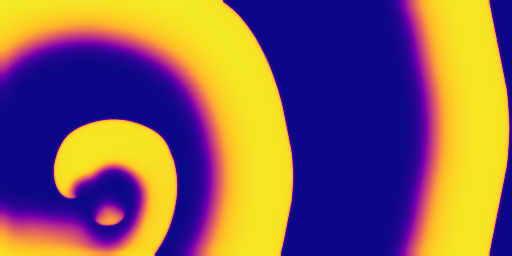
\includegraphics[width=\textwidth]{breakup-40}
        \vspace{-\baselineskip}
        \caption{2000 steps}
    \end{subfigure}
    \begin{subfigure}[b]{.3\textwidth}
        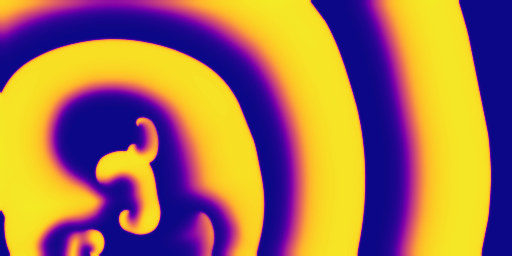
\includegraphics[width=\textwidth]{breakup-60}
        \vspace{-\baselineskip}
        \caption{3000 steps}
    \end{subfigure}
    \begin{subfigure}[b]{.3\textwidth}
        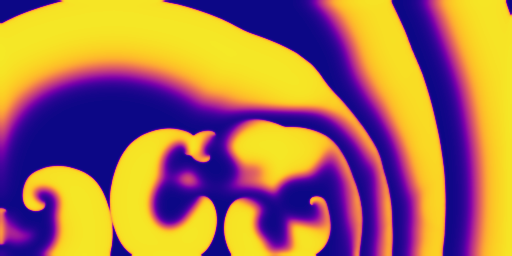
\includegraphics[width=\textwidth]{breakup-90}
        \vspace{-\baselineskip}
        \caption{4500 steps}
    \end{subfigure}
    \begin{subfigure}[b]{.3\textwidth}
        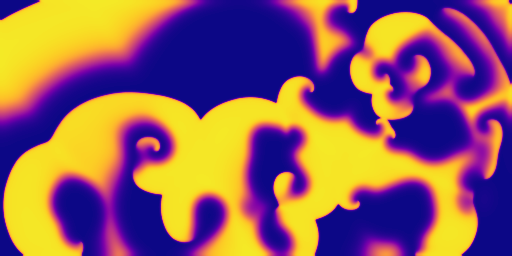
\includegraphics[width=\textwidth]{breakup-120}
        \vspace{-\baselineskip}
        \caption{6000 steps}
    \end{subfigure}
    \begin{subfigure}[b]{.3\textwidth}
        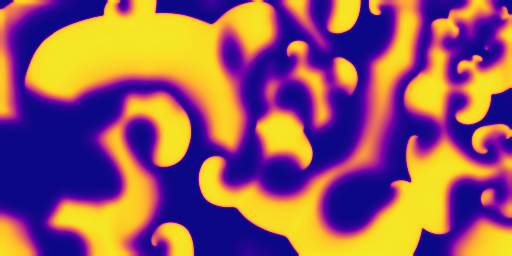
\includegraphics[width=\textwidth]{breakup-150}
        \vspace{-\baselineskip}
        \caption{7500 steps}
    \end{subfigure}
    \label{fig:breakup}
    \caption{Image series of spiral wave breakup due to tip-wake interaction}
\end{figure}

With the Aliev-Panfilov model the aforementioned initial conditions generate
an ever-growing spiral without any disruptive behaviour.


% vim: set ff=unix tw=79 sw=4 ts=4 et ic ai :
